\documentclass[letterpaper,10pt,titlepage,draftclsnofoot,onecolumn,onesided] {IEEEtran}
\usepackage{listings}
\usepackage{underscore}
\usepackage[bookmarks=true]{hyperref}
\usepackage[utf8]{inputenc}
\usepackage[english]{babel}
%\usepackage{titling}
\usepackage{graphicx}
\usepackage{xcolor}
\usepackage[noadjust]{cite}
\usepackage{setspace}
\usepackage{float}
\usepackage{pdfpages}
\nocite{*}
\graphicspath{ {img/} }
%\usepackage{abstract}

\newcommand{\namesigdate}[2][4cm]{%
  \begin{tabular}{@{}p{#1}@{}}
    #2 \\[2\normalbaselineskip] \hrule \\[0pt]
    {\small \textit{Signature}} \\[2\normalbaselineskip] \hrule \\[0pt]
    {\small \textit{Date}}
  \end{tabular}
}
\newcommand{\studentnamesigdate}[2][4cm]{%
  \begin{tabular}{@{}p{#1}@{}}
    #2 \\[2\normalbaselineskip] \hrule \\[0pt]
    {\small \textit{Signature}} \\[2\normalbaselineskip] \hrule \\[0pt]
    {\small \textit{Signature}} \\[2\normalbaselineskip] \hrule \\[0pt]
    {\small \textit{Signature}} \\[2\normalbaselineskip] \hrule \\[0pt]
    {\small \textit{Signature}} \\[2\normalbaselineskip] \hrule \\[0pt]
    {\small \textit{Date}}
  \end{tabular}
}

\hypersetup{
    bookmarks=false,    % show bookmarks bar?
    pdftitle={Progress Report},    % title
    pdfauthor={Cramer Smith, Sam Lichlyter, Eric Winkler, Zach Schneider},                     % author
    pdfsubject={Progress Report},                        % subject of the document
    pdfkeywords={IFT, Report, Postal}, % list of keywords
    colorlinks=true,       % false: boxed links; true: colored links
    linkcolor=black,       % color of internal links
    citecolor=black,       % color of links to bibliography
    filecolor=black,        % color of file links
    urlcolor=blue,        % color of external links
    linktoc=page            % only page is linked
} 

\lstdefinestyle{customperl}{
  belowcaptionskip=1\baselineskip,
  breaklines=true,
  frame=L,
  xleftmargin=\parindent,
  language=Perl,
  columns=fullflexible,
  showstringspaces=false,
  basicstyle=\footnotesize\ttfamily,
  keywordstyle=\bfseries\color{green!40!black},
  commentstyle=\itshape\color{purple!40!black},
  identifierstyle=\color{blue},
  stringstyle=\color{orange},
  numbers=left
}
\lstset{escapechar=@, style=customperl}

% Document Title:
\def\doctitle{A Tool to Visualize the Structure of a Codebase Using Information Foraging Theory Design Patterns}
\def\doctype{Final Report}
\def\team{Team Postal | Group \#38}

\markboth{Oregon State University}{\doctitle}

\begin{document}

\title{\Huge{\bfseries{\textsf{\doctitle}}}\\\textsf{\Large{\doctype}}\\\textsf{\large{\team}}}
\author{Cramer Smith, Sam Lichlyter, Eric Winkler, Zach Schneider}

\maketitle
\vfill

\setlength\parindent{0pt} \textbf{Abstract:} Developer tools are often complex pieces of software. 
Gathering and manipulating useful information for a programmer can often be a slow and costly process. 
By implementing Information Foraging Theory design patterns in the creation of these tools, the information collected may be more useful or produced faster. 
Information Foraging Theory is the theory and math behind the choices people make to maximize the value of the information they find versus the cost of getting that information.
The aim of this project is to develop a tool that will act as a proof of concept to this idea and increase developer efficiency.
Through the implementation of multiple IFT design patterns, the Postal team will create a developer tool that helps enforce and maintain code structure. 

\vfill

\pagebreak

\tableofcontents


\pagebreak

\section{Introduction}
\subsection{Client and Project Origins}
This project originated in August 2016 when one of the the team's members, Sam Lichlyter, was made aware of a research opportunity offered by Professor Christopher Scaffidi from Oregon State University. 
Prof. Scaffidi's primary research area is in Information Foraging Theory (IFT) which revolves around studying how humans find and utilize information sources. 
Sam, already a student researcher under Prof. Scaffidi, asked if he could create a Senior Capstone project out of IFT in a new study concerning software developers.
Prof. Scaffidi prompted Sam to identify a team and to come up with a project proposal that would develop a software tool according to the principles of IFT. 
Sam included Eric Winkler, Zach Schneider and Cramer Smith in the potential Capstone team. 
There were two proposals submitted for consideration: an interface to allow developers to read and search program log files more easily, and an extension for an IDE that would automatically organize a developers code into appropriate concerns i.e., the data layer, interface layer, and application layer.
The latter of the proposals was selected and this Capstone team was formed to undertake it.

\subsection{Project Purpose and Expectations}
A more detailed explanation of what the team was tasked with is as follows.
First, design a tool according to IFT design patterns that will help developers find and utilize information, in this case, within an IDE.
Second, build and code said tool until it is in a state where it is useful in its main purposes.
Next, organize a series of formal user tests to determine if the tool aides developers in performing a set of real world tasks.
Finally, analyze the results of the tests and, if the results are positive, write a formal research paper describing the entire process and its relationship to IFT.
Prof. Scaffidi supervised the design process in the Fall. The team met with him about once and month to check in and discuss any design questions or changes. 
Emails were exchanged a bit more often. 
He left the coding and implementation phase largely up to the team during the end of Fall through the Winter and contact was infrequent. 
Spring term saw contact pick up again as the team finalized the product with him and began arranging the necessary materials for user testing. 
Prof. Scaffidi has and will continue to directly facilitate the actual testing and analysis process until it is complete.

\subsection{Project Roles}
Throughout the year, each team member assumed and carried out various roles depending on the stage of the project. 
Every member generally contributed to all aspects of the project, but the responsibility for some areas was assumed primarily by one individual.

Sam undertook served as the team's primary client contact since the relationship had existed prior to the beginning of this project. 
He had a major role in the design and implementation of the parser component of this tool, along with Eric. 
Additionally, Sam wrote many of the grammars and rules that the parser would use to find specific data within developers' codebases. 

Zach took primary responsibility for project documentation, deadlines and general administrative work. He contributed to early iterations of the data structure used to store parsed data within the tool. 
He then transitioned to adding features to the user interface (UI) and testing various use cases within it.

Cramer did much of the research into which IDE the tool would be developed for. 
Once Visual Studio Code was decided upon by the team as the platform for this project, he also created the core of code required to launch and include extensions within that platform. 
Cramer deployed each iteration of the tool to the Microsoft VS Code Extension Gallery online when various project milestones were reached.

Eric served as overall project architect, coming up with the general structure of the project from the original proposal and changing it as necessary throughout the year. 
He worked with Sam in building the parser and created the core of the UI and Electron window code. 
When the parser was modified in the middle of the year, he also re-worked the data structure system being used. \\


\section{Original Requirements and Timeline}
The original Requirements Document for this project is inserted in the following pages.
\includepdf[pages={-}]{requirements.pdf}
\pagebreak
\section{Updates to Requirements and Timeline}
Below is a simplified list of all requirements for this project as of the final Requirements document submitted on November 4th, 2016. 
No changes to requirements were made for the duration of the project.
\subsection{Product Functions}
\small{
\begin{center}
	\begin{singlespace}
		\begin{tabular}{ |  p{0.25\linewidth}  |  p{0.25\linewidth}  | p{0.25\linewidth} | p{0.25\linewidth} |}
		\hline
		0 & Requirement & Changes & Comments \\ \hline
		
			1
		& 
			\begin{itemize}
				\item Offered in a free, cross-platform text editor
			\end{itemize}
		& 
			\begin{itemize}
				\item None
			\end{itemize}
		&
			\begin{itemize}
				\item Completed
			\end{itemize} 
		
        \\ \hline

			2
		& 
			\begin{itemize}
				\item Provide the user with a visual perspective of their project
			\end{itemize}
		& 
			\begin{itemize}
				\item None
			\end{itemize}
		&
			\begin{itemize}
				\item Completed
			\end{itemize} 
		
        \\ \hline

            3
		& 
			\begin{itemize}
				\item Parse project for bad coding practice/incorrect formatting
			\end{itemize}
		& 
			\begin{itemize}
				\item None
			\end{itemize}
		&
			\begin{itemize}
				\item Completed, This is implemented through the Notifications/Error grammars.
			\end{itemize} 
		
        \\ \hline

            4
		& 
			\begin{itemize}
				\item Indicate to user when \"errors\" are parsed
			\end{itemize}
		& 
			\begin{itemize}
				\item None
			\end{itemize}
		&
			\begin{itemize}
				\item Completed, Mid-winter we began to refer to errors by a more appropriate name, notifications. 
                The functionality remained unchanged.
			\end{itemize} 
		
        \\ \hline

        	5
		& 
			\begin{itemize}
				\item Visually display links between files
			\end{itemize}
		& 
			\begin{itemize}
				\item None
			\end{itemize}
		&
			\begin{itemize}
				\item Completed
			\end{itemize} 
		
        \\ \hline

        	6
		& 
			\begin{itemize}
				\item Rules defined by user defined grammars
			\end{itemize}
		& 
			\begin{itemize}
				\item In an earlier, pre-final version of the requirements documents, rules were defined by W3 best practices for web projects.
                This changed by the time of our final submission on November 4th to rules being defined by user grammars.
			\end{itemize}
		&
			\begin{itemize}
				\item Completed
			\end{itemize} 
		
        \\ \hline

        	7
		& 
			\begin{itemize}
				\item Ignore lines of code marked in an exception list
			\end{itemize}
		& 
			\begin{itemize}
				\item None
			\end{itemize}
		&
			\begin{itemize}
				\item Completed, Implemented through comment grammars and the postal.ignore functionality.
			\end{itemize} 
		
        \\ \hline

        	8
		& 
			\begin{itemize}
				\item Parse projects up to 100,000 LOC with less than one second of lag
			\end{itemize}
		& 
			\begin{itemize}
				\item None
			\end{itemize}
		&
			\begin{itemize}
				\item This requirement is situationally completed. 
                It does work for projects of 100,000 lines but will have problems with individual files of that size.
			\end{itemize} 
		
        \\ \hline
		\end{tabular}
	\end{singlespace}
\end{center}
}
\subsection{External Interfaces}
\small{
\begin{center}
	\begin{singlespace}
		\begin{tabular}{ |  p{0.25\linewidth}  |  p{0.25\linewidth}  | p{0.25\linewidth} | p{0.25\linewidth} |}
		\hline
		0 & Requirement & Changes & Comments \\ \hline
		
			1
		& 
			\begin{itemize}
				\item Two main elements: File Map UI and Error List
			\end{itemize}
		& 
			\begin{itemize}
				\item None, some additionally functionality was added.
			\end{itemize}
		&
			\begin{itemize}
				\item Completed, Error List now refereed to as Notification List
			\end{itemize} 
		
        \\ \hline

			2
		& 
			\begin{itemize}
				\item Toolbar for options
			\end{itemize}
		& 
			\begin{itemize}
				\item None
			\end{itemize}
		&
			\begin{itemize}
				\item Completed
			\end{itemize} 
		
        \\ \hline

            3
		& 
			\begin{itemize}
				\item Populate File Map with contents of opened solution
			\end{itemize}
		& 
			\begin{itemize}
				\item None
			\end{itemize}
		&
			\begin{itemize}
				\item Completed, This is implemented through the Notifications/Error grammars.
			\end{itemize} 
		
        \\ \hline

            4
		& 
			\begin{itemize}
				\item Visual indicator of links and errors
			\end{itemize}
		& 
			\begin{itemize}
				\item None
			\end{itemize}
		&
			\begin{itemize}
				\item Completed
			\end{itemize} 
		
        \\ \hline

        	5
		& 
			\begin{itemize}
				\item /"Dig down/" into a file to identify sub-nodes
			\end{itemize}
		& 
			\begin{itemize}
				\item None
			\end{itemize}
		&
			\begin{itemize}
				\item Completed
			\end{itemize} 
		
        \\ \hline

        	6
		& 
			\begin{itemize}
				\item Error list displays all errors parsed
			\end{itemize}
		& 
			\begin{itemize}
				\item None
			\end{itemize}
		&
			\begin{itemize}
				\item Completed
			\end{itemize} 
		
        \\ \hline

        	7
		& 
			\begin{itemize}
				\item User can click error to navigate to corresponding location in code
			\end{itemize}
		& 
			\begin{itemize}
				\item None
			\end{itemize}
		&
			\begin{itemize}
				\item Completed, Implemented through double clicking a node
			\end{itemize} 
		
        \\ \hline

        	8
		& 
			\begin{itemize}
				\item User can hover over error and will highlight location in File Map
			\end{itemize}
		& 
			\begin{itemize}
				\item None
			\end{itemize}
		&
			\begin{itemize}
				\item Completed
			\end{itemize} 
		
        \\ \hline
		\end{tabular}
	\end{singlespace}
\end{center}
}

\subsection{Functions}
\small{
\begin{center}
	\begin{singlespace}
		\begin{tabular}{ |  p{0.25\linewidth}  |  p{0.25\linewidth}  | p{0.25\linewidth} | p{0.25\linewidth} |}
		\hline
		0 & Requirement & Changes & Comments \\ \hline
		
			1
		& 
			\begin{itemize}
				\item Be able to parse JavaScript, HTML and CSS
			\end{itemize}
		& 
			\begin{itemize}
				\item None
			\end{itemize}
		&
			\begin{itemize}
				\item Completed, implemented through user grammars
			\end{itemize} 
		
        \\ \hline

		\end{tabular}
	\end{singlespace}
\end{center}
}

\subsection{Performance Requirements}
\small{
\begin{center}
	\begin{singlespace}
		\begin{tabular}{ |  p{0.25\linewidth}  |  p{0.25\linewidth}  | p{0.25\linewidth} | p{0.25\linewidth} |}
		\hline
		0 & Requirement & Changes & Comments \\ \hline
		
			1
		& 
			\begin{itemize}
				\item 30 HTML, 5 CSS, 10 JS files in less than one second
			\end{itemize}
		& 
			\begin{itemize}
				\item None
			\end{itemize}
		&
			\begin{itemize}
				\item Completed
			\end{itemize} 
		
        \\ \hline

		\end{tabular}
	\end{singlespace}
\end{center}
}


\subsection{Software System Attributes}
\small{
\begin{center}
	\begin{singlespace}
		\begin{tabular}{ |  p{0.25\linewidth}  |  p{0.25\linewidth}  | p{0.25\linewidth} | p{0.25\linewidth} |}
		\hline
		0 & Requirement & Changes & Comments \\ \hline
		
			1
		& 
			\begin{itemize}
				\item Available on VS Code Extension Marketplace
			\end{itemize}
		& 
			\begin{itemize}
				\item None
			\end{itemize}
		&
			\begin{itemize}
				\item Completed
			\end{itemize} 
		
        \\ \hline

		\end{tabular}
	\end{singlespace}
\end{center}
}

\subsection{Gantt of Implementation Progress for the Year}
\begin{figure}[H]
	\centering
	\includegraphics[width=.75\textwidth]{Gantt}
	\caption{Gantt of the implementation progress for the academic year.}
\end{figure}
\begin{figure}[H]
	\centering
	\includegraphics[width=.75\textwidth]{GanttTop}
	\caption{Top half of the Gantt for readability.}
\end{figure}
\begin{figure}[H]
	\centering
	\includegraphics[width=.75\textwidth]{GanttBottom}
	\caption{Bottom half of the Gantt for readability.}
\end{figure}

% Your original design document, as well as a discussion of what had to change over the course the year.
\section{Design Document and Changes}
\includepdf[pages={-}]{design.pdf}
\subsection{Discussion of Changes}
The original design of the Visual Studio Code extension was targeted towards web developers.
Discussions with the client transitioned this viewpoint to make the tool more universal and available to a wider audience of developers.
The tool was then redesigned to allow for broader customization through the use of ``grammars'' which users can use to define certain behaviors for the extension.
This change allowed for more customization and tuning available to the user, meaning it didn't really matter what kind of developer they were because they could adapt the tool to their needs.\\

Another change from the original design was the use of certain technologies which will also be discussed below.
The developers had intended to use the programming language Perl and associated libraries to parse the project directories of the user but found keeping the entire project written in TypeScript made more sense and was easier to implement while keeping the same amount of functionality. 
Other technology changes included using a custom implementation of the features provided by jQuery's Advanced News Ticker API library.\\

One major design change from the original document was not parsing the updated file on save or having multiple versions of the parsed data structure around.
It was decided to only parse the project directory when the user explicitly said to (when the user wanted to refresh the file map UI or notification list). \\

% Your tech review, in its original form. Did you change your mind about any technologies? What had to change?
\section{Technology Review and Changes}
\includepdf[pages={-}]{techreview.pdf}
\subsection{Discussion of Changes}
Sam Lichlyter discussed the different parser technologies the project would use to parse the files in the user's project directory.
He started out with the parser class.
It was decided the developers would use a custom parser for the reasons he mentioned in the original Technology Review. \\

The third section Sam talked about was specifically which Perl parsing tool the team would use.
At this point in designing and developing the extension the team was pretty convinced they were going to use Perl as their parsing language.
The design change mentioned above where they transitioned the target audience from web developers to a wider audience of developers moved them away from using Perl.
Perl had a lot of libraries and built in functions specifically to parse HTML which the extension still needed to do, but it was decided it was better to design a more universal parser.\\

Zach Schneider then went on to talk about how the extension would store it's data.
He mainly talked about different types of databases including SQL and NoSQL databases.
It was decided the team wouldn't use a database at all but rather implement the data structure using a single JSON file which could then be passed to the UI to read to generate the appropriate visualization. \\

As mentioned above in the design changes, the developers decided to not keep two or more versions of the parsed data, so there was no need to have a technology that compared them. \\

Cramer Smith looked at different Integrated Development Environments (IDE) and their respective event listeners and languages they are written in to allow the developers a better experience building the tool for that specific IDE.
The developers decided to use Visual Studio Code for the IDE they would build the extension for.
They did this for the reasons mentioned in the original Technology Review.\\

The team decided to transition to built in events instead of using EventEmitter for the event listeners.
Because the extension is only launched and the directory parsed when the user explicitly tells it to, there was no need for more complicated event listeners than the ones already built in. \\

Eric Winkler discussed the different ways to build and show the UI. 
The team decided to use vis.js as the main JavaScript engine for displaying the nodes and edges within the file map UI.
The broken rules (now called notifications) was planned on being displayed using jQuery's Advanced News Ticker API. 
This was overruled by custom code as the News Ticker API didn't add much value in terms of usefulness of the extension.
The actual location of the file map UI was decided to be done within an Electron window.\\

\section{Weekly Blog Posts}
	\input{blogposts}	
		
	

\section{Engineering Expo Poster}
%leave this blank, we'll just print this out separately in color

\section{Project Documentation}
\subsection*{Cramer Smith}
% Cramer, This is Your PARTY! I wrote this to myself.
This section of the document covers the details of the projects implementation, and the ways that the user can expect to install and use the tool.

% How does your project work?
\subsection{How It Works}
The extension consists of three main pieces. The first, and most complicated, is the parser. 
The second is the visualization, and the third is the IDE Visual Studio Code.
The user starts in IDE opening a code project. 
From the VSC IDE the user can start the extension, and then the parser gets to work on the users code. 
The parser is responsible for breaking the users code down into informational data structure that the visualizer can use to generate the map that the user can then navigate. 

The parsing is done in several steps. 
It is implemented using a combination of functions built into VSC as well as some custom code using Node.js. 
The built in functions in VSC are mainly involve getting all the files in the user's current working directory. 
The custom code is the bulk of the parser.
It is written in typescript and uses a number of Node.js modules, and it is responsible for checking the file for the things specified within the grammars that are supplied by the user. 
A grammar is a JSON object defined by the user and consists of regex patterns to define  rules that the parser uses when creating the visualization file map. 
The parser then takes this grammar and generates a datastructure. 
The file map based on the defined links between files, or whatever the user specifies within the grammars.
The map consist of nodes and sub-nodes that are representations of the files and their connections that the parser created.
The map is shown on the visualization custom UI. \\

\begin{figure}[H]
	\centering
	\includegraphics[width=.75\textwidth]{InformationERDEPS-eps-converted-to}
	\caption{Control flow of the way the data structure is formed}
\end{figure}

On execution of a Visual Studio Code command, the Electron application will activate the parser generate the file map. 
The visualization is done in the separate Electron window that is opened.
It has several things to display from the parser information. 
The main piece of information that the visualization displays is the file map and other information is the notification list. 
The file map is a graphic representation of the of the user's project solution. 
It appears as a hierarchical graph of interconnected nodes where the nodes represent a file or directory in the user's project directory, and an edge represents some link (defined in the parser section) between the two files. 
The location of the nodes in the hierarchy will reflect its position in the project's directory. 
This web will feature nodes of different sizes and will allow the user to zoom and pan the view. 
The size of the node is based on the number of links to that object.
A color corresponding to the type of file. 
Color values are based on the VSC color scheme for aesthetic reasons.
The name of the node is retrieved from the file struct name field and is displayed as text beside the node. 
A red circle will appear on the node if there are notifications within the FileStruct for that node. 
In other words, if the size of the notification array within the FileStruct is not zero. 
The file map is rendered within its own div using the vis.js library 'Network' module. 
The Library by default includes the rendering, panning and zooming functionality. \\

The other piece of the projects custom UI is the notification list. 
The notification list will display all notifications currently in the project directory in the form of a vertical list. 
These notifications will be retrieved when the UI opens from the same data structure is being generated. 
These notifications will be retrieved in a per node fashion and will also be grouped in the error list in the same order.
The notifications list will exist to the side of the file map in the same electron application screen. 
The list will allow the user to scroll when the number of errors result in the list exceeding the electron window height.
When a notification in the list is hovered over, these errors highlight the corresponding node in the file map by changing the color value of said node.
When a notification in the list is clicked, the extension will open the file in Visual Studio Code?s text editor and scroll to line where the notification location exists. 
The notification list is in its own div and scrolling functionality is achieved through the use of jQuery Advanced News Ticker. \\ % is it? 

\begin{figure}[H]
	\centering
	\includegraphics[width=.75\textwidth]{UpdatedDataStruct-eps-converted-to}
	\caption{Information that is stored in the data structure and the way that is it interpreted by the custom UI and displayed}
\end{figure}

Data handling within the Postal Extension consists of three main entities or processes: the data structure, serialization of the data structure and the storage of the data structure in a JSON file.
The data structure is a dictionary of file nodes, stored as JavaScript objects. 
These JavaScript objects come from the Parser parsing the currently loaded project for links and notifications.
The data structure can be considered the live version of the project data, as its data structure is updated by the parser every time the project is parsed. 
The nodes changed in the data structure will then be serialized into JSON jQuery using the JSON.stringify function built into JavaScript. 
This JSON will be saved to a file, which can further be read by the Electron UI functions for updating the project node and notifications visualization. \\

Now onto the IDE. 
There are two main interactions that happens the specific IDE events the opening of the custom extension UI and the interfacing network that allows the user to click on the custom UI in electron and have events happen in the VSC interface. 
The first of these events is opening the custom extension UI, this is done by creating a new process that runs the Electron window and passing the information that the parser has collected to that process.  
The interfacing network is opened and closed every time the user clicks a UI element within the custom UI. 
The network is a simple server client network with the server being the VSC IDE and the client being the Electron window. 
The VSC initializes itself as a server that will listen for the Electrons message when the user interacts with a UI Element. 
Once that happens the extension will navigate the users code window on VSC to the appropriate location that the user specified when they clicked on the custom UI.  \\

% What is its structure?
\subsection{Structure}

The extension is developed with a Model View Controller design.
The Model being a data structure that is created by the parser. 
The View being the custom UI displays a visualization of the data structure.
The controller is the communication between the data structure and the UI.

\begin{figure}[H]
	\centering
	\includegraphics[width=.75\textwidth]{MVCsimple}
	\caption{Diagram of the way the Model View Controller Design is implemented}
\end{figure}

% Theory of operation: is a description of how a device or system should work
\subsection{Theory of Operation}

Once installed and with the proper grammars made for the project that the user is working on the extension should function as follows. 
The user can then use the command \texttt{command + shift + p} to open the command dialogue.
From there the user can input the \texttt{Postal} command. 
This operation will start the parsing of their files, and the creation of the custom UI that will open soon after inputting the command. 
Within the custom UI the user can navigate around the representation of their code using their mouse and zoom functionality.
They will be able to view different code elements based on the grammars they have defined.
The user is also able to view the notification list. 
The user can click on any of the nodes or any of the notifications and they will be navigated back to the VSC window where a new tab will be opened and the area in the code that was specified by the element clicked will be displayed, and ready for the user to edit.
The user is able to access and edit their custom grammars in the settings.json file that is part of VSC. 


% How does one install your software, if any?
\subsection{Installation}

\subsubsection{From Visual Studio Code Marketplace}
\begin{enumerate}
	\item	Within Visual Studio Code, click the extensions tab (the last one that looks like a block)
	\item 	type "postal" into the search bar
	\item 	click the install button
	\item 	Navigate to: \texttt{~/.vscode/extensions/postal-team.postal-\$version/}
	\item 	Run the command \texttt{npm install}
	\item 	Navigate to: \texttt{~/.vscode/extensions/postal-team.postal-\$version/lib/app}
	\item 	Run the command \texttt{npm install}
\end{enumerate} 

\subsubsection{From GitHub} Run the following commands:
\begin{enumerate}
	\item 	\texttt{git clone https://github.com/slichlyter12/Postal.git}
	\item 	\texttt{cd postal}
	\item 	\texttt{npm install}
	\item 	\texttt{cd lib/app}
	\item 	\texttt{npm install}
	\item 	\texttt{cd ../..}
	\item 	\texttt{code .}
	\item 	VSCode should now be open with Postal's source code
	\item 	Hit F5
	\item 	Navigate to: \texttt{~/.vscode/extensions/postal-team.postal-\$version/}
	\item 	Run the command \texttt{npm install}
	\item 	Navigate to: \texttt{~/.vscode/extensions/postal-team.postal-\$version/lib/app}
	\item 	Run the command \texttt{npm install}
\end{enumerate}

% How does one run it?
\subsection{Run Instructions}

To run the extension once it is properly installed all on has to do is open VSC and open a project. 
From there the user uses the \texttt{Command + Shift + p} command and the VSC command dialogue will be open, and the user can then input the command \texttt{Postal} and the Postal Extension will start.

% Are there any special hardware, OS, or runtime requirements to run your software?
\subsection{Prerequisites}

To use the extension the user needs to have Visual Studio Code and be able to use the npm installer.
To be able to run the npm install means that they have to have Node.js installed. 
They need this for the commands that are described in the Installation section.
This is needed because the extension uses Electron to display the map that the extension builds, and Electron is too large to package and have put on the Visual Studio Code Extension Marketplace.


\section{Resources and Technologies}

The most complex technologies the team had to learn was Node.js and vis.js

\subsubsection{Node.js}
For learning Node we primarily used the Electron reference guide available here: 
\hyperref{https://electron.atom.io/docs/}
This was the most helpful resource in figuring out how to build an extension for Electron as well as basic node process information. 
The section on the Electron API was especially helpful.
\\
The team also made use of a couple github projects for reference purposes. 
The biggest help by a wide margin was the VSCode Color Picker made by Anseki.
\hyperref{https://github.com/anseki/vscode-color/}
While the code was quite dense it was also essential in figuring out how to launch an Electron window from VSCode. 
It also gave the team some insight in how to better build the high-level structure of our extension. 
It is important to note that the team did not take any code from the project and only referred to it as a guide for using the correct Node and Electron functionality.

\subsubsection{Vis.js}
Vis.js is intuitive for doing basic things with graph visualizations. 
However, it can be very clunky when trying to implement more complex behaviors on top of its standard functionality. 
The main resources used for figuring out Vis.js related difficulties were the official documentation and examples webpages.
\url{http://visjs.org/docs/network/}
\url{http://visjs.org/network_examples.html}
The documentation itself was helpful for more specific information like finding function overloads but was not at all useful for understanding how to use Vis.js's functionality. 
Fortunately, Vis.js also provided a very comprehensive examples page with samples demonstrating the majority of supported functionality and function usage.

\subsubsection{Additional Resources}
We also made use of other technology specific websites and Stack Overflow for minor issues.
Both Regex101 and Curious Concept's JSON formatter were very helpful tools.
\url{https://regex101.com/}
\url{https://jsonformatter.curiousconcept.com/}
Additionally, we based the majority of our parser’s architecture on the compiler we built in CS480. 
It was, in retrospect, surprising how useful that class was to completing this project.


\section{Learning and Overall Experience}
% What technical information did you learn?
% What non-technical information did you learn?
% What have you learned about project work?
% What have you learned about project management?
% What have you learned about working in teams?
% If you could do it all over, what would you do differently?

\subsection{Sam Lichlyter}
\subsubsection{What technical information did you learn?}
Since my main source of income over the past seven years or so is as a web developer, I am extremely familiar with JavaScript.
However, I had never used TypeScript before, which is essentially Microsoft's version of JavaScript that has a few added functionalities, including types.
I found this extremely helpful as one of my main complaints with JavaScript is that it is not typed.
I also learned how to use Node.js which I had been meaning to do for quite some time.
I had never heard of Electron before which was pretty useful to be able to essentially write a website that would be run as it's own application in it's own window.
This project also turned out to be a compilers crash course.
The parser we wrote was essentially a customizable compiler, so I learned a lot of the intricacies of how those work.\\

\subsubsection{What non-technical information did you learn?}
I think one of the biggest things I learned was how much I appreciated some of the things we were taught in the very beginning of our college career that I more or less disregarded when they were first introduced to me.
The big one that stands out is paired-programming.
I don't think this project would have been as successful as it was or completed in the timeframe needed without paired-programming.
Eric and I were able to successfully do this by him ``directing'' and me ``driving.''
I was able to focus on the syntax and typing while Eric was able to basically tell me how everything was connected.
If we had tried to do this on our own I don't think either of us would have been able to keep straight what had to be connected to what and we would have run into hours of debugging later down the road. \\

Another big thing I am now more appreciative of is designing before coding.
They tell us this all throughout our college career, but usually our assignments aren't big enough to warrant this kind of design first approach.
This project however definitely was.\\

\subsubsection{What have you learned about project work?}
Piggy-backing a bit off of the last section, designing first is extremely important.
Especially for projects of this magnitude and bigger like I expect a lot of professional jobs will have us work on.
Our team didn't completely disregard designing the system before we started, we just didn't quite know what we needed, so it made it extremely difficult to design thoroughly. \\

\subsubsection{What have you learned about project management?}
One of the biggest takeaways from this project about managing a team is communication.
It is extremely important that everyone is on the same page, and everyone knows what the end goal is.
This is something we ran into at least once.
At one point we were all on one page and our client was on another, and at another point some of us were on one page and the others were on a different page.
Keeping everything straight in a system like this is complicated, but everyone needs to know their roles and how they fit into the bigger picture of getting the whole team to where they want to be.\\

\subsubsection{What have you learned about working in teams?}
This wasn't quite something I learned through this project but it was definitely exemplified in this project.
And that was that everyone on the team has their own strengths and weaknesses.
Some people are better at doing research into different technologies, others are better at conceptualizing large and complicated systems.
These are things that are vital to each team and that team should use these abilities and talents to their full extent. \\

Another important aspect I learned about working in teams was that separating business from pleasure is very important. 
At the end of the day you all want to be friends but still have a really cool project to show off to people.
You need to be able to separate personal feelings from what needs to get done, and then when the work is over, you need to not really talk about work until the appropriate time.
For me at least, I found this very helpful to maintain the friendships I had with the people on my team.\\

\subsubsection{If you could do it all over, what would you do differently?}
If I would do it all over again, I would go through the advice I just listed above and implement it.
I would put more effort into design first before implementation, make sure everyone knows their roles in the team and how they fit into the bigger picture, use the things we were taught in school for how they're meant to be used, etc. 

\subsection{Zach Schneider}
\subsubsection{Technical Information Learned}
The core development of this project involved the learning and utilization of many new technologies, languages, and programming principles for the team and myself.
I had previously used VS Code, but had never developed an extension for it or any other Electron based code editing platform.
Debugging an add-on and testing it on all relevant platforms is not only useful practice for future projects in that vain, but also gives me a great appreciation for the work other developers have done over the years in extending the tools I use and enjoy.
This was my first foray into using TypeScript, a JavaScript super-set that includes types and class-based object oriented programming. I enjoyed working with TypeScript, and felt like it included many of the JavaScript programming strategies I'm familiar with while offering a more consistent and featured experience.
TypeScript was primarily utilized in programming for our Node.js server within VS Code.
I had used Node in one project previously, but our capstone project this year gave me a much more in depth view into how Node servers work and how to effectively program with them.
Additionally, I learned and became proficient in the Latex document preparation system.
Latex creates consistent, professional looking documents, and I used it to create most of the documentation and reports for this project.

\subsubsection{Non-Technical Information Learned}
During this project I became more proficient in writing up formal documentation, particularly in adherence to IEEE standards. 
Learning how these kinds of documents are developed, updated and referenced will greatly aide me in all future programming jobs.
I also believe my writing ability improved overall, as the many different reports required for this class stretched me in ways I hadn't previously been challenged to attempt.
I learned how to merge the writing styles of others within a single paper in order to have a more cohesive submission that flows, instead of 4 separate sections pasted into one document.
Editing, while not re-writing is a skill of mine that has certainly been furthered while working on this project.

\subsubsection{Project Work}
Perhaps the most significant thing I learned about project design and implementation is how important it is for the designers and implementers to be on the same page.
Even in our case where each of our team members served both roles, we had quite a few problems early on in not understanding what design or project feature the others were trying to convey to us.
Sometimes we mistakenly wrote code in an entirely different train of thought than other sections, leading to serious conflicts in our project's structure and function.
Ultimately, our solution was increased communication and more time put into the planning stages of each component's section.
Along these lines, our team struggled to even conceptualize what we wanted from our project as a whole and if our concepts would actually work.
In a few cases, we wrote a design or specification for a feature, then realized while creating that feature that the original envisionment would not work out.
What I can take away from this is, again, how important the planning and design stages of projects are to their success.
Experience in working on projects like ours will help when starting on new projects in the future.

\subsubsection{Project Management}
One of the issues our project faced was running out of time at deadlines. 
Even if they were self-established deadlines, we couldn't strike a balance of having a deadline be significant while also flexible enough to accommodate series design problems that we occasionally encountered.
My time management in these contexts was certainly tested in trying to allow for enough time to accomplish what was needed while also not setting deadlines too far into the future.
Additionally, I learned the importance of differentiating when a feature or task should be done versus when it needs to be done. 
Setting these standards for myself and communicating them to my team effectively contributed positively to my knowledge of project management.

\subsubsection{Working in Teams}
Team work can often be difficult - personality clashes, differences in work ethic, lack of communication - these are all fairly expected when working on team projects. 
While our team was generally able to learn and work through many of these standard issues, a unique circumstance we possessed was that we are all friends outside of school.
Some of us had heard to warnings to not work with friends on projects, but we didn't really pay them heed.
Throughout this project, it has been exceedingly difficult to draw the line between our work relationships and our social relationships. 
Often we would finish up work on the project then promptly spend the rest of the weekend hanging out.
While this led to an easy dynamic early on, our relationships became strained when serious problems occurred, such as individuals not meeting deadlines, not communicating or forgetting about meetings.
Though our project worked out in the end, this experience is not one that I'd like to undertake with friends again.
In the future I will aim to let friends be friends and work colleagues be work colleagues.

\subsubsection{What I Would Do Differently}
With the aforementioned lessons being learned, if I were to do this project again, I would do a few things differently.
First, I would not choose to work with close friends on an extended and stressful project such as this.
I would make sure to spend a more significant amount of time in the early stages really nailing down what the project's purpose, goals, design and features will be.
Communication about these plans would be made with the team and our client much more frequently at the beginning.
Coding would begin in early December instead of January, as the extra month of working through bugs would make a large difference in final quality and lessen deadline stress along the way.
Finally, I would begin utilizing user testing far earlier, even before features are complete in order to get feedback and save the team some of the re-writing that occurred in the later phases of the project.
Despite these changes I would make, I feel the majority of the project went well and I'm proud of the result.

\subsection{Cramer Smith}

\subsubsection{Technical Information Learned}

This was the largest project that I have ever made, and we wrote it in JavaScript and TypeScript. 
I learned a lot about JavaScript and Node.js.
I learned the usefulness of code organization. 
I always knew that having well organized code was good, but I had never had a long term large project that really needed it.
It was great after we had done a major part of the development adding smaller features to the tool was much easier because we already had all these small pieces well put together and these parts could easily be put together to make something larger.
I also learned about thenables. 
Thenables are a very annoying and incredibly flexible way of working with asynchronous function calls.
I had never used TypeScipt and for any function that was not working as I expected is because it was probably running asynchronously. 
To fix it I quickly learned that a thenable was needed.
I also learned about using a client server relationship to communicate between processes.
To get the user events between the custom UI with the Electron window and the VSC editor we needed to communicate between two different processes. 
I always though that processes were very closed off entities, and they are unless you tell the processes to communicate to one another. 
To do that communication I set up the client server.

\subsubsection{Non-Technical Information Learned}

I learned some self confidence.
Usually in team project I do not try to be the idea man. 
I have always assumed that others are smarter than me, but this project I learned that I have some good ideas.
So I tried to make myself more heard during this project.

\subsubsection{Project Work}

It is a lot of work to get a big project working, and a lot of work can be saved by a good initial design.
We had an okay initial design. 
The core ideas of that initial design are still there, but some of that design did not work as expected. 
We had to redo a lot of work because of the initial design was not sufficient.
But even if we had had a perfect design it would still have been a lot of work. 
The amount of hours that we put in to get the tool working, was more than I thought it would be. 

\subsubsection{Project Management}

Communication is extremely important. 
I knew that before.
It was really evident though when we initially delegated the separation of work between the four of us, and we all started developing without talking too much to one another. 
Then by the time we were all supposed to be done with our respected parts we came together and none of the parts worked together. 
We should have been talking with each other more in that crucial development phase.
That being said
I think I would have liked some more structure with the way we all managed the project. 
It was nice when we nominated the team leader to handle all the document deadlines.
It was nice to know that if I was unsure of what I needed to do for X document I could ask Zach.
That was the only real structure that we had though. 	

\subsubsection{Working in Teams}

It is hard to not have emotions rise.
There were times when it was very tense in out Slack chat. 
I am still not sure how to remedy this problem.
I think it would be different in a professional environment.
I delegation is good, but only with really good communication.
There needs to be a good understanding of the expectations of the team.
 
\subsubsection{What I Would Do Differently}

Besides the differences that I stated in the above sections I wouldn't be in a team with my friends. 
I think this hurt my friendships with these people, and I was probably less motivated because I knew my friends would be more forgiving. 



\subsection{Eric Winkler}

\subsubsection{Technical Information Learned}
From a technical perspective, I've learned about or become more proficient in:
\begin{itemize}
    \item JavaScript and TypeScript
    \item Node.js
    \item Electron
    \item Vis.js
    \item Git and Github
    \item Other Web-technologies (HTML, CSS)
    \item Software Design
    \item Asynchronous design
    \item Object oriented Programming
    \item Debugging
    \item Compilers
    \item Using APIs in general
    \item Reading Documentation
\end{itemize}

\subsubsection{Non-Technical Information Learned}
The theme to the non-technical lessons I learned while work on this project is that I have a new appreciation for a ton of things I learned here but hadn’t used in a practical way before.
\\
To start with, I now love paired programming. 
Building the Parser and back-end of this project was potentially the most complicated thing I have attempted during my undergraduate career. 
It was almost necessary to have Sam writing code while I focused on keeping track of what exactly we were doing and what we still had to do. 
Writing most of the code together probably saved us tens of hours.
\\
I also learned to love classes. 
I've never had to use classes on the basis of trying to abstract complex problem but being able to describe things in terms classes and forget about lower level details was very helpful.
\\
Finally, I learned to appreciate the importance of designing before coding. 
I'm not sure I've ever completed a homework assignment by first design it and the writing the code. 
Everything had been, relatively speaking, simple to implement. 
However, without an assignment guide or anyone to hold our hand through the process, we were forced to actually draw out the components of the system and really think about why we were implementing things the way we were.
I think the most valuable piece of non-technical Information I gained from this project would be that I really like to do design related work. 
I may attempt to pursue a career path where I can do more architecture and systems design than programming, provided that exists. 

\subsubsection{Project Work}
The most valuable lesson about project work I learned is that if a group plans on splitting the work into separate modules and assigning one or more modules exclusively per person, the modules should still be designed together as a group. 
The team has mentioned this problem before in previous documents and it should be mentioned again how important it is to have well defined interfaces. 
What I've never brought up is that those interfaces imply that the design and functionality of the two modules are clearly defined and understood by the team.
That's the more important lesson to note. 
It doesn't matter at all what the exact specifications of the interfaces are if there is missing or overlapping functionality in those modules. 
If I had to come away with only one important lesson from this project it would be this: design thoroughly with all members of the team present.

\subsubsection{Project Management}
From a project management perspective, I've learned the importance of setting one's own deadlines and setting them early. 
Around the middle of winter term, the team concluded that we were starting to fall behind of where we wanted to be in terms of implementation progress. 
We had made the decision to get a working build of our extension on the VSCode store by the next coming Monday. 
Nothing was specifically due for the class but we had placed this artificial deadline on ourselves because of concern that something might cause problems if we had planned to be finished by the end of the term instead. 
Because of the how tight our deadline was, we forced ourselves to work close to 36 hours within a three-day period. 
During that crunch we discovered serious problems with our design that would have caused the project to be a failure if we had waited much longer.
My opinion is that deadline may have saved the project.

\subsubsection{Working in Teams}
I was fortunate to work with an excellent team. 
Everyone was motivated and completed their assignments on time. 
We had no major problems and communication was consistent. 
One lesson I learned is that it helps quite a bit to have at least one person who can act as a leader. 
This person doesn't necessarily have to delegate jobs or roles, but having an individual to check on team member's progress and keep a general level of organization is beneficial. 

 
\subsubsection{What I Would Do Differently}
A problem the team had that we don't reflect on much is that we had a bit of miscommunication on project priorities with our client. 
We had spent so much time on our back end figuring out how to get our parser working consistently that we had neglected the front end quite a bit. 
In a meeting our client was not happy with our progress, though a substantial amount had been made since our last check in. 
We had failed to realize that as a tool, it was only as good as it was usable, i.e. its front end. 
I regret not frequently communicating with our client and making him a larger part of the process.


\pagebreak
\section{Appendix 1}
\subsection{Code Samples}
	\subsubsection{Example Grammar}
	This is the default grammar that parses HTML and PHP files for divs and links.
	
	\begin{lstlisting}
{
    "id" : 0,
    "title" : "html",
    "filetypes" : ["html", "php"],
    "rules" : [{
            "title": "div",
            "type": "tagged",
            "options" : {
                "tagStart": "<div",
                "namedOption" : "id=\"(.+?)\"",
                "tagEnd": ">",
                "closingTag": "</div>",
                "nodeColor": "blue"
            }
        }, {
            "title": "href link",
            "type" : "link",
            "options" : {
                "link": "href=[\"](.+?)[\"]",
                "nodeColor": "blue"
            }
        }, {
            "title": "includes link",
            "type": "link",
            "options": {
                "link": "include=[\"](.+?)[\"]",
                "nodeColor": "blue"
            }
        }, {
            "title": "body",
            "type": "tagged",
            "options" : {
                "tagStart": "<body",
                "tagEnd": ">",
                "closingTag": "</body>",
                "nodeColor": "blue"
            }
        }
    ]
}
	\end{lstlisting}

	\pagebreak
	\subsubsection{Recursive Get All Links}
	This function grabs all the links from the data structure of a specified file struct and it's children.
	\begin{lstlisting}
// Recursive function to get all links from this and children
function getAllLinksFromFileStructRecursive(FileStructID) {
    var links = [];

    // check parent
    if (DFS[FileStructID].links.length > 0) {
        for (var i = 0; i < DFS[FileStructID].links.length; i++) {
            var link = DFS[FileStructID].links[i];
            links.push(link);
        }
    }

    // check children
    if (DFS[FileStructID].subContainers.length > 0) {
        var childLinks = [];
        for (var i = 0; i < DFS[FileStructID].subContainers.length; i++) {
            var childFileStructID = DFS[DFS[FileStructID].subContainers[i].toFileStructid].id;
            childLinks = getAllLinksFromFileStructRecursive(childFileStructID);

            // push what we found to parents link list
            for (var j = 0; j < childLinks.length; j++) {
                links.push(childLinks[j]);
            }

        }
    } 

    return links;
}
	\end{lstlisting}

\pagebreak
\section{Appendix 2}	
\subsection{Images}
	\begin{figure}[H]
		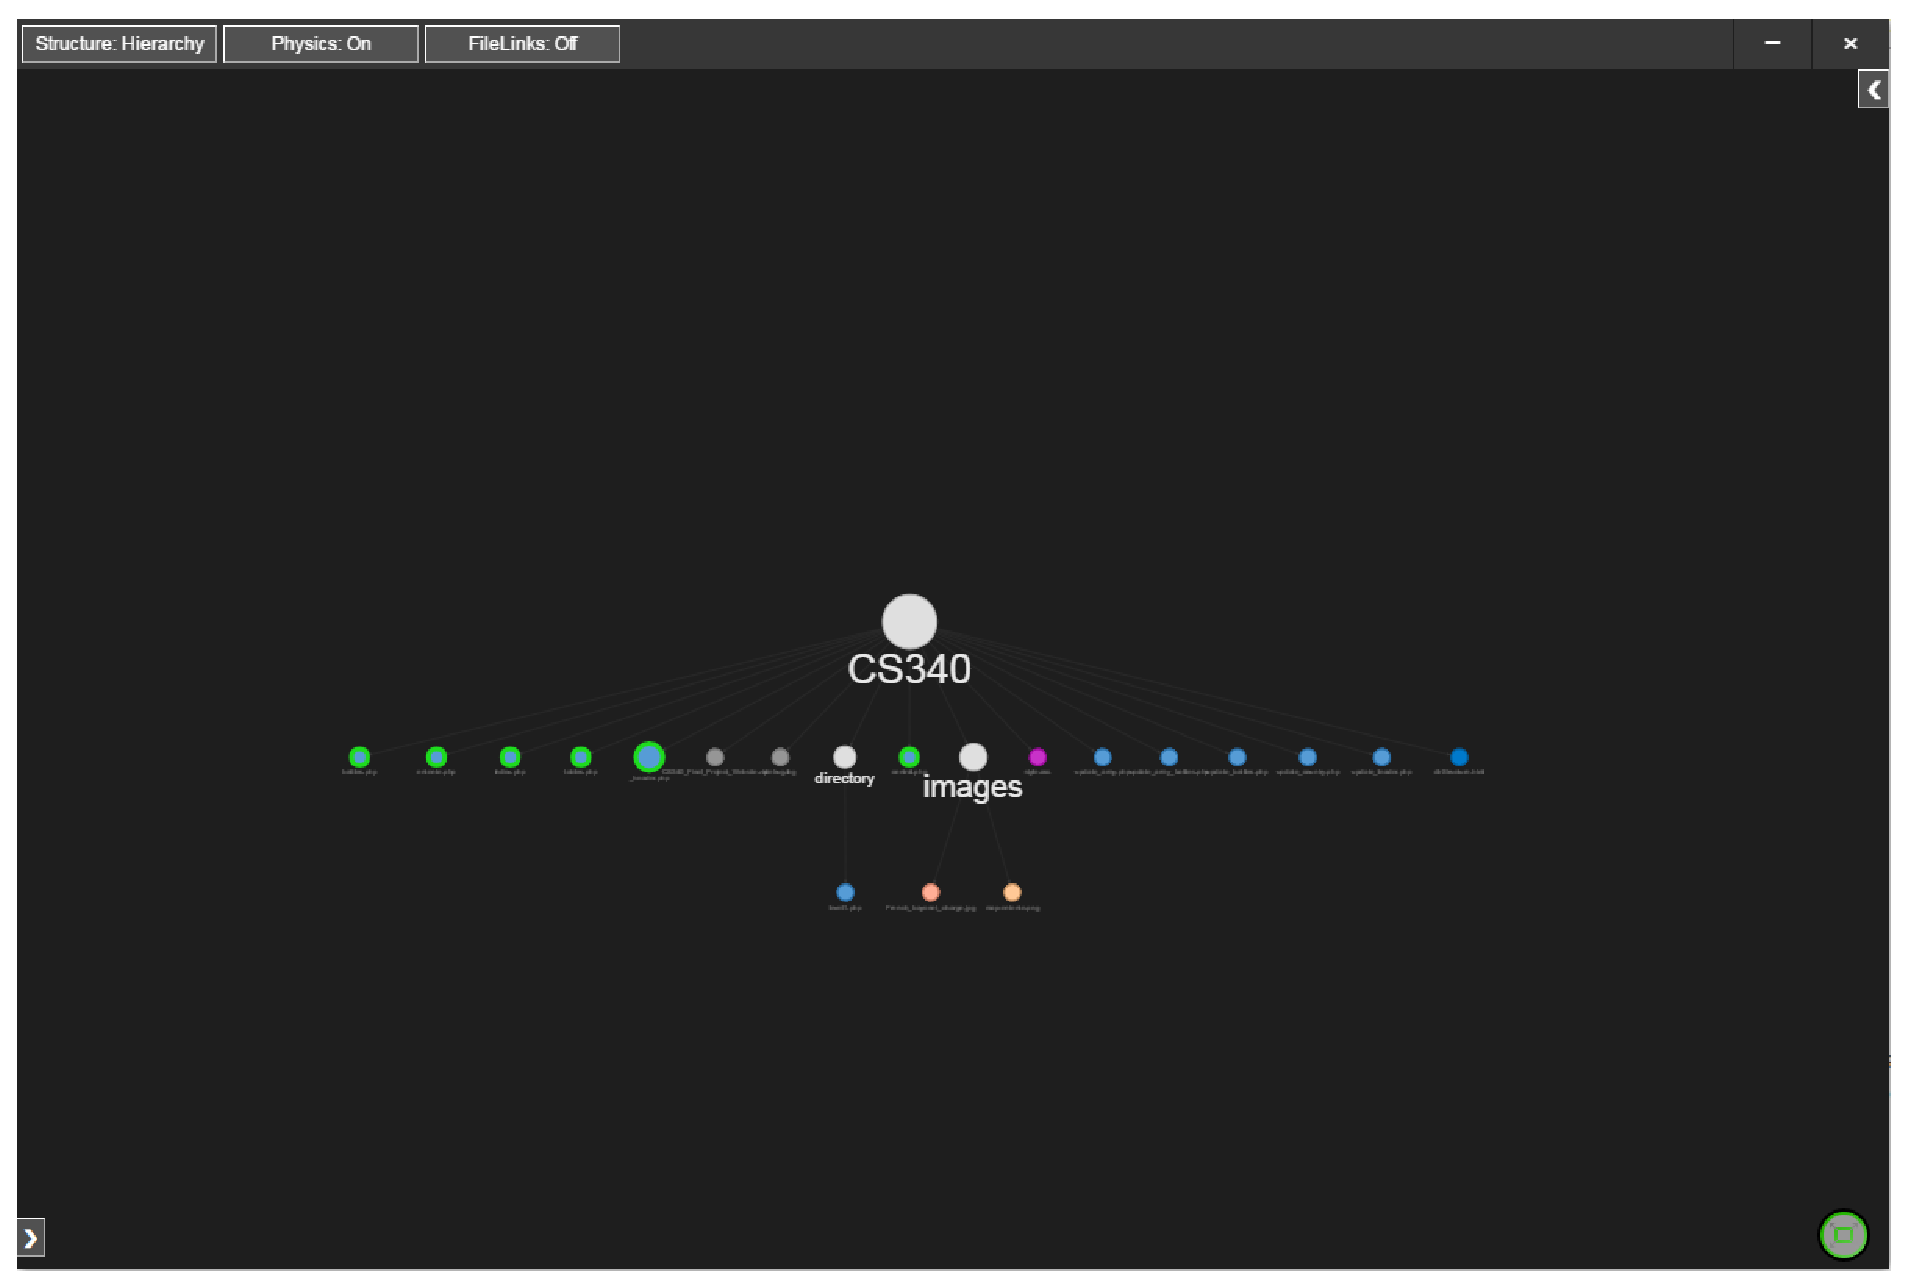
\includegraphics[width=400px]{PostalUI}
		\caption{Visualization Interface}  
	\end{figure}
	
	\begin{figure}[H]
		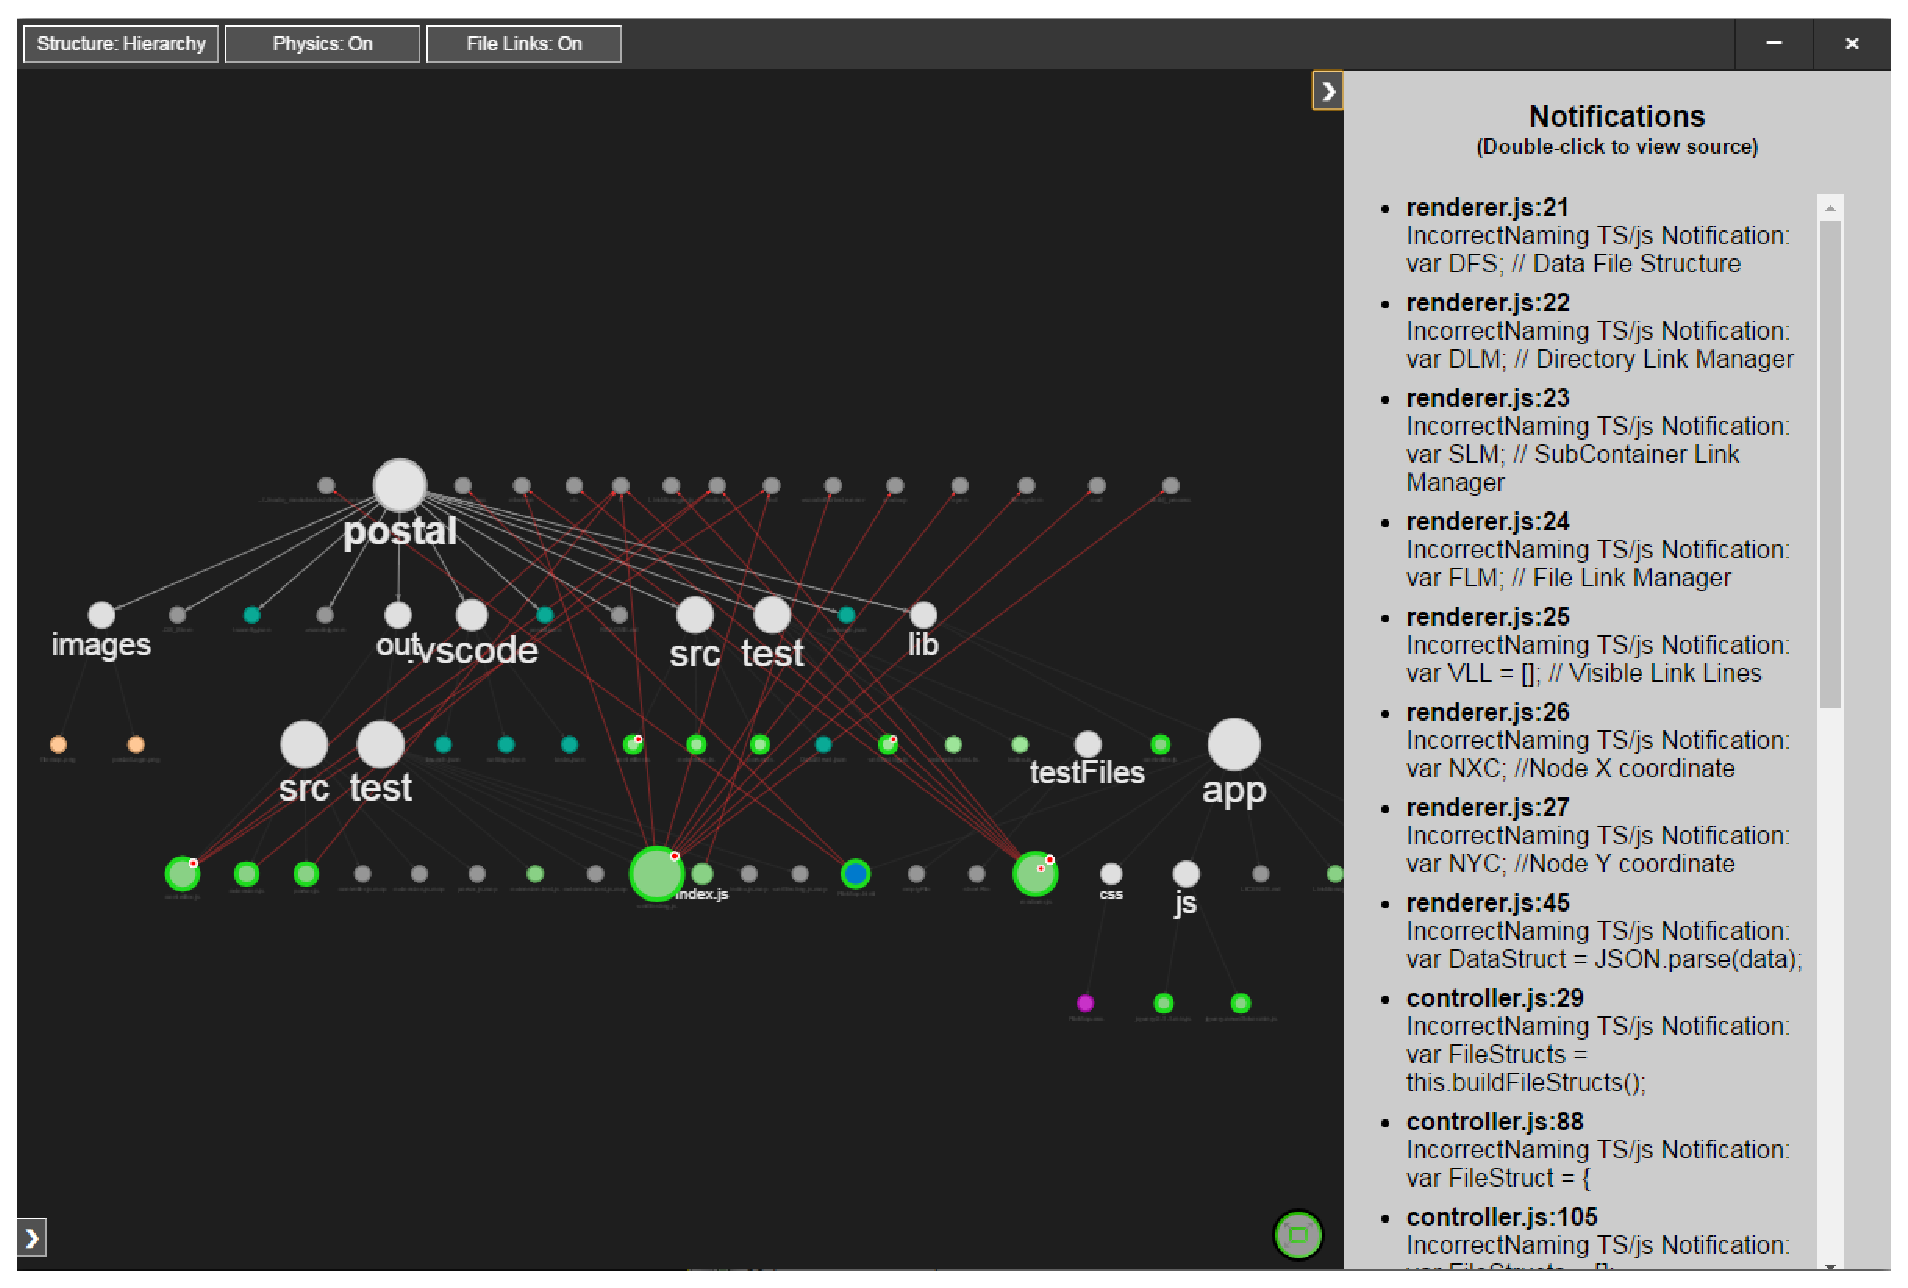
\includegraphics[width=400px]{PostalNotification}
		\caption{Notification Interface}  
	\end{figure}
	
	\begin{figure}[H]
		\includegraphics[width=400px]{UpdatedDataStruct}
		\caption{Updated Data Structure}
	\end{figure}
	
\pagebreak
\bibliographystyle{IEEEtran}
\bibliography{progress-report-team38}


\end{document}

